\documentclass[twocolumn,12pt,a4paper]{article}

\usepackage[english]{babel}
\usepackage[utf8]{inputenc}
\usepackage[T1]{fontenc}
\usepackage{multicol}
\usepackage[top=3cm, bottom=3cm, left=2.5cm, right=2.5cm]{geometry}
\usepackage[bookmarks=true,bookmarksnumbered=true,hidelinks]{hyperref}
\usepackage{fancyhdr,lastpage}
\renewcommand{\footrulewidth}{0.4pt}
\usepackage[bf,sf]{titlesec}
\usepackage[font={footnotesize,sf}]{caption}
\usepackage{siunitx}
\usepackage{titling,graphicx}
\usepackage{abstract}
\usepackage{amsmath}
\usepackage{siunitx, minted}

\pagestyle{fancy}
\lhead{\textsf{Solar Sailing from Earth to Mars}}
\rhead{\textsf{Team 891}}
\cfoot{\thepage{} of \pageref*{LastPage}}

\setlength{\columnsep}{1.5cm}

% Numerar equacions amb la secció
\numberwithin{equation}{section}

\author{\textsf{Team 891}}
\title{\textsf{\textbf{Problem A: Solar Sailing from Earth to Mars}}}
\date{\textsf{November 12, 2017}}
\makeindex

\begin{document}
\renewcommand{\abstractname}{}
\renewcommand{\absnamepos}{empty}
\begin{titlingpage}
 \maketitle

\noindent \hrulefill \\
\begin{abstract}
Test test test

\end{abstract}
\hrulefill \\

\end{titlingpage}

\begin{titlingpage}
\tableofcontents
\end{titlingpage}

\section{Introduction}

\subsection{Approach}
The motion of a solar sail within the Solar System, after a number of assumptions have been made, can be modeled by a set of relatively concise differential equations. Therefore, the problem at hand essentially becomes an initial value problem. 

As a first approximation, it can be found that a solar sail moves following as a logarithmic spiral. We used this fact to determine the feasibility of a trip from Earth to mars using solar sail propulsion, and to give a lower bound on the size of the sail for this trip to take a reasonable amount of time.

However, more complexity needed to be introduced to the model in order to understand the later stages of the trip, namely, from the point when the gravitational pull of Mars is no longer negligible. This means that the equations are no longer solvable analitically, so numerical methods must be used.

 A more detailed interpretation of the problem was needed so that a more precise model could be built. Understanding firstly the physical foundations around solar sailing was essential in order to perform an accurate analysis. Research has been done on the different forces affecting the sail for trajectories to be computed. Since some initial conditions are already given it has been necessary to verify whether these were the best options to accomplish the overall goal of the study or not.
 
  Moreover the aim of the survey is not only to calculate the path followed by the craft but also to determine its velocity so that a safe landing can be guaranteed. However, as trying to consider the attraction of Mars does not always give accurate results, this is not an easy task, though an estimate of craft arrival to Mars is presented at the end.
 
 It will be understood that the sail starts its trajectory with a radial velocity equal to the Earth's escape velocity, and with a tangential velocity equal to the Earth's linear velocity around the Sun. 
 
The release of the space craft will be considered at the time in which the Earth is closest to Mars, although, as it will be further discussed, results do not point in this being the best configuration. Since orbits of both planets are regarded as circular, as mentioned in the following section, this occurs when the Earth, Mars and the Sun are aligned.

The main goals of the article are to discuss a suitable distribuiton of the mass of the space craft, as well as to simulate possible trajectories and the arrival of the sail to Mars.

\subsection{Main assumptions}
To model the motion of a solar sail, we assumed it to be subject solely to the gravitational attraction from the Sun and solar radiation pressure. This yields a meaningful first approximation which can be used to gain insight on 

Throughout the article, several assumptions have been made, both as interpretations of the problem and in order to facilitate the model. However, all assumptions are supported by literature, and all the approximations were found to be reasonable. We present the approximations and interpretations made.

\begin{itemize}
\item The orbits of Mars and the Earth are coplanar and perfectly circular.
\item The only forces acting on the sail during its flight are the gravitational force exerted by the Sun and the thrust given by the inciding photons. Since the initial radial velocity is the Earth escape velocity, it is reasonable not to consider its attraction. In a first approach to the model, Mars attraction force has not been computed.
\item As stated in the problem given, we assume the total mass of the space craft is \SI{2 000}{kg} , including the payload and the sail. Thus, our goal is to maximize the payload while still finding a reasonable time of flight. 
\item Comparing the research which has already been done to the fact that the preassure exerted by light is twice its energy density, one finds that the case given is one of a perfect reflection.
\item We assume the only initial tangential velocity of the sail is the Earth's linear velocity. Thus, one ignores the effects of the Earth's rotation.
\end{itemize}

\subsection{General assumptions}
When one considers the general model of a solar sail orbiting the Sun, one finds that the acceleration of the center of mass of the sail-Sun system is non-vanishing, and therefore, taking the center of mass as the origin of the reference frame, as we do in subsequent calculations, does not yield an inertial frame. However, this acceleration is negligible and so we use the approximation that the acceleration of the center of mass of the Sun-sail system ---which can in turn be approximated by the Sun's position--- is zero.

Furthermore, the differential equations we derive assume that the sail is solely under the influence of the Sun's gravitation and radiation. The sail, however, is to be released at escape velocity from the Earth. This means that it will move in exactly the same way it would if the Earth were not there. 

Finally, for this model to be applicable, the orbits of the Earth and Mars must be assumed circular and coplanar, and the sail is assumed to remain perpendicular to the plane of the orbits.

\section{The physics of solar sailing}
We will follow \cite{tsu} and \cite[Ch. 4]{mcinnes} for most of this section.
\subsection{Radiation pressure}
It is well-known that electromagnetic wave carries an energy density. The fundamental idea behind solar sails is to use this energy as a means of propulsion in a way very much similar to how traditional sails take advantage of the kinetic energy of the wind. Given that the diameter of any reasonable solar sail will be much smaller than its distance to the Sun, one may approximate the solar radiation that arrives at the sail in the form of sinusoidal planar waves of frequency \( \omega \).

If \( E(t) \) is the amplitude of such waves, then the energy density, \( u \), they carry is given by \( u = \epsilon_0 E(t)^2 = \epsilon_0 E_0^2 \cos^2{\omega t} \). If one averages this over a period \( T \), then one obtains that the average energy density is simply \( \epsilon_0 E_0^2 /2 \), which can be rewritten as \( I/c \), where \( I \) is the intensity of the wave and \( c \) is the speed of light. Thus one finds that the pressure that incoming radiation exerts on the sail is \( I/c \). However, given that the material of the sail is not a black body, a fraction, \( R \), of the absorbed radiation will be emitted, giving rise to an additional term of pressure of the form \( RI/c \). If the sail is made out of a perfectly reflective material then it is the case that \( R = 1 \) and then the total pressure exerted on the sail is \( p = 2I/c \). This is the case for the problem at hand.

The intensity of a spherical wave is inversely proportional to the square of the distance from the source. Thus, the force exerted on the sail by the radiation from the Sun follows an inverse square law. We can make this dependence explicit by considering the equality \( Ir^2 = I_0 r^2_0 \), where \( I_0 \) is the intensity of solar radiation at a distance equal to the radius of the orbit of the Earth, \( r_0 \). And so we find that the force due to radiation pressure on a sail of surface area \( S \) is
\begin{equation}
 	\mathbf{F}_R(r) = \dfrac{2SI_0r_0^2}{c}\dfrac{1}{r^2} \mathbf{\hat{e}}_r \label{eq:radiation force}
\end{equation}

\subsection{Equations of motion for a solar sail: orthogonal case}
We have established that a solar sail that receives radiation in a direction orthogonal to itself experiences an inverse square central force. The other force acting on the sail is gravitational attraction due to the Sun ---we will consider the gravitational pull from other planets to be negligible when compared to that of the Sun---, which is also an inverse square force law. Namely:
\begin{equation}
 	\mathbf{F}_G(r) = -\dfrac{G M_S m}{r^2} \mathbf{\hat{e}}_r \label{eq:gravitational force}
\end{equation}
where \( m \) is the mass of the solar sail ---including the mass of the payload--- and \( M_S \) is the mass of the Sun.

Thus, we are now in a position to write the equations of motion for the solar sail
\begin{align}
	a_{r} &= \dot{v}_r - \dfrac{v_{\theta}^2}{r} = \dfrac{F_R - F_G}{m} \label{eq:equations of motion perpendicular} \\
	a_{\theta} &= \dot{v}_{\theta} + \dfrac{v_r v_{\theta}}{r} = 0 
\end{align}
It is common to introduce a number of parameters to better encapsulate the nature of a solar sail. The characteristic acceleration of a solar sail, \( a_R \), is defined to be the acceleration the sail experiences due to radiation pressure at a distance equal to 1 astronomical unit (AU) from the Sun. In keeping with the notation introduced in the previous section we write
\begin{equation} \label{eq:characterisit acceleration}
  a_R = \dfrac{2SI_0}{mc}
\end{equation}
It is then immediate to see that, if we denote the acceleration due to radiation pressure by \( a_R \) we have
\begin{equation}
  a(r) = a_R \dfrac{r_0^2}{r^2} 
\end{equation}
We can do the same with the acceleration due to gravity and we find
\begin{equation}
  a(r) = a_G \dfrac{r_0^2}{r^2} = \dfrac{G M_s}{r_0^2} \dfrac{r_0^2}{r^2}
\end{equation}
With this in mind we can then rewrite \autoref{eq:equations of motion perpendicular} as follows
\begin{align} \label{eq:equations of motion characteristic accelerations}
  \dot{v}_r - \dfrac{v_{\theta}^2}{r} &= (a_R - a_G) \left(\dfrac{r_0}{r}\right)^2 \\
	\dot{v}_{\theta} + \dfrac{v_r v_{\theta}}{r} &= 0
\end{align}
As we have already mentioned, this shows that the motion of a solar sail receiving radiation orthogonal to itself is governed by an inverse square law. In particular, the sail will move as if it were orbiting a star with a mass less than the Sun.

\subsection{Equations of motion for a solar sail: general case}
This, however, is only true if the sail is orthogonal to the incoming radiation. Indeed, if we allow for the sail to be at an arbitrary orientation, then its tangential acceleration is no longer zero. For this, we introduce the angle \( \alpha \), which is the angle between the vector normal to the sail, \( \hat{\mathbf{n}} \), and the radial direction. We do not allow for full freedom of the sail, and assume that its normal vector remains in the plane that contains the radial vector and is orthogonal to the sail itself. Now, the force due to radiation pressure has two contributions. The incoming photons exert a force that is now proportional to the orthogonal projection of the sail onto the radial direction, therefore of \( IS\cos{\alpha}/c \). This force is in the radial direction. The emitted photons exert a force that has the same modulus, but given that the sail behaves like a mirror, they are emmited in the direction orthogonal to the radial direction, and so the force due to the outgoing radiation is proportional to \( {-\hat{\mathbf{e}}_{\theta}} \). So we have
\begin{equation}
  \mathbf{F}_R(r) = \dfrac{2IS \cos{\alpha}}{c} ( \hat{\mathbf{e}}_{r} - \hat{\mathbf{e}}_{\theta})
\end{equation}
We now observe that because of symmetry, the vector \( \hat{\mathbf{e}}_{r} - \hat{\mathbf{e}}_{\theta}  \) is proportional to \( \hat{\mathbf{n}} \), and, because \( \hat{\mathbf{n}} \) is a unit vector then we have \( \hat{\mathbf{e}}_{r} - \hat{\mathbf{e}}_{\theta} = \cos{\alpha} \hat{\mathbf{n}} \). 
And thus we obtain
\begin{align}
  \mathbf{F}_R(r) &= \dfrac{2IS \cos^2{\alpha}}{c} \hat{\mathbf{n}} \\
									&= \dfrac{2IS \cos^2{\alpha}}{c} (\cos{\alpha} \hat{\mathbf{e}}_r + \sin{\alpha} \hat{\mathbf{e}}_{\theta}) 
\end{align}

Finally, we can rewrite the equations of motion for a solar sail in this more general case as follows:
\begin{align} \label{eq:equations of motion general case}
  \dot{v}_r - \dfrac{v_{\theta}^2}{r} &= (a_R \cos^3{\alpha} - a_G) \left(\dfrac{r_0}{r}\right)^2 \\ 
  \dot{v}_{\theta} + \dfrac{v_r v_{\theta}}{r} &= -a_R	\sin{\alpha} \cos^2{\alpha} \left(\dfrac{r_0}{r}\right)^2
\end{align}
As a consistency check, we note that if \( \alpha = 0 \), that is, the sail is orthogonal to the radiation, we recover \autoref{eq:equations of motion characteristic accelerations}. However, the equations we have just obtained are \emph{not} the equations for a particle experiencing central force motion.   

\section{Model analysis and results}
\subsection{First model}
Making an aproximation for the radial velocity will enable solving explicitly the motion equation. This will provide the survey of a first general outcomes.

\subsubsection{Feasibility of the trip}
To solve \autoref{eq:equations of motion general case} it is common to assume \( \dot{v}_r = 0\), as done in \cite{tsu} and \cite{mcinnes}. With this assumption the equations become those of a logarithmic spiral. Then \( v_r = \dot{r} \) can be isolated and then integrated to find an expresssion for the time of travel between two circular and coplanar orbits of a given radius in terms of only the parameters \( \alpha \), \( a_R \) and \( a_G \):

\begin{equation} \label{eq:time of flight between orbits}
	t=\frac{1}{3}\cdot\frac{r_0^{3/2}-r^{3/2}}{r_0\sqrt{a_R}}\cdot\frac{(a_G/a_R-\cos^3\alpha)^{1/2}}{\sin\alpha\cos^2\alpha}
\end{equation}

Therefore, assuming that the orbits of Mars and the Earth are indeed coplanar, we can compute the time it would take for a solar sail to complete the trip from Earth to Mars, for a given choice of parameters. \autoref{fig:logarithmic spiral} shows an approximation of the trajectory the sail follows.

\begin{figure}
	\centering
	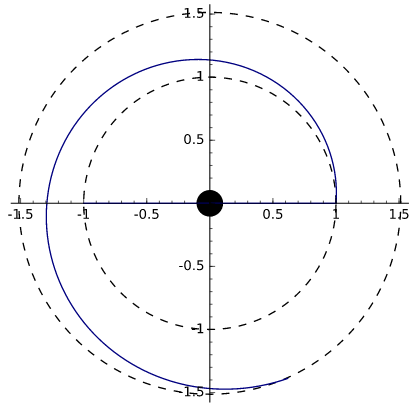
\includegraphics[scale=0.5]{espiral.png}
	\caption{First approximation of the sail trajectory, in blue. The Sun is in the middle and the dashed lines represent the orbits of the Earth and Mars. Axis in AU.}
	\label{fig:logarithmic spiral}
\end{figure}

Given the data in the problem then \( a_G \) is completely determined and has a value of \SI{5,928e-3}{m \cdot s^{-2}}. The characteristic acceleration can be rewritten in terms of the mass of the sail, \( m_s \):
\begin{align*}
  a_R &= \dfrac{2I_0}{c} \dfrac{S}{m} \\
  		&= \dfrac{2I_0}{c} \dfrac{m_s}{\sigma m}
\end{align*}
where \( \sigma \) is the surface density of the sail, as given in the problem. And so we find that \( a_R = \num{6,45e-7} m_s \) using the value for \( I_0 \) given in \cite{hollerman}.

As for the sail angle \( \alpha \), by minimizing \autoref{eq:time of flight between orbits}, it can be seen that the optimum angle depends only on the ratio \( a_R / a_g \) which is commonly called the lightness parameter of the sail and denoted by \( \beta \) With the values obtained for the characteristic accelerations, the value for \( \beta \) is \( \num{e-4} m_s \). Nevertheless, for values of \( \beta \) up to 0.5, which is the range that is accessible in this situation given that \( m_s \) cannot exceed \SI{2000}{kg}, the optimum angle shows very litle variation from 35.26º, as can be seen in \autoref{fig:optimum angle}, which shows the value of the factor dependent on \( \alpha \) in \autoref{eq:time of flight between orbits}.

\begin{figure} 
	\centering
	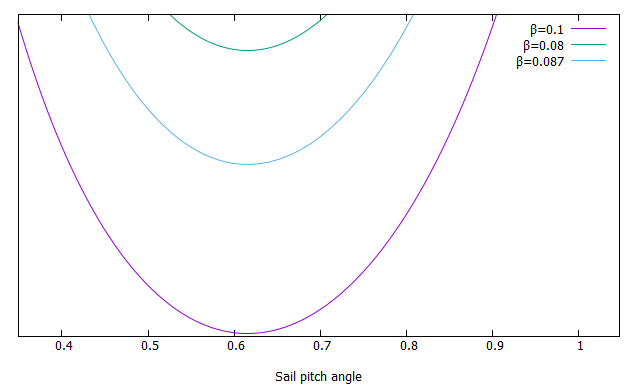
\includegraphics[scale=0.3]{angle.png}
	\caption{Dependence of flight time on the sail angle $\alpha$}
	\label{fig:optimum angle}
\end{figure}

To test the feasibility of the voyage, we will compute the time of flight as a function of the mass of the sail from Earth's orbit to Mars' with the optimum sail angle. The results are shown in \autoref{fig:time of flight}

Of course, there is no sail mass which produces an optimum time, since allotting more mass to the sail only affects \( a_R \), and not \( a_G \), which is mass-independent. 

\begin{figure}[b]
	\centering
	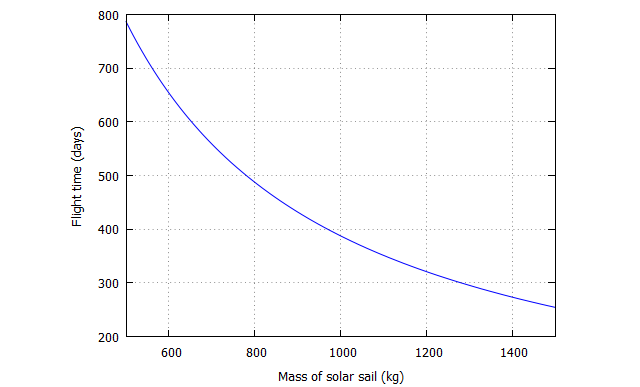
\includegraphics[scale=0.35]{time}
	\caption{Flight time as a function of the sail mass}
	\label{fig:time of flight}
\end{figure}

With a total available mass of \SI{2000}{kg}, a manned mission propelled with a solar sail is obviously not possible. The purpose of a solar sail would then be to send unmanned cargo to Mars, possibly satellites or rovers to explore its surface. According to \cite{presskit}, the Mars Science Lab (MSL) mission, which sent the rover Curiosity to Mars, had a total mass of \SI{3893}{kg}. The rover itself, however had a mass of \SI{899}{kg}, and most of the remaining mass of the mission was destined to propulsion systems. Given that a hypothetical solar sail propelled mission would have no need for fuel tanks or propulsion systems, it seems reasonable that a payload mass of \SI{1000}{kg} would suffice to carry a rover or similar device to Mars. This would leave another \SI{1000}{kg} to be used for a sail of area \SI{142857}{m^2}. As such, the total time to travel to Mars in these conditions is of approximately 390 days. Again, comparing with a mission such as MSL, which took 254 days to reach Mars, we find that this time is higher, but the potentials savings in fuel and propulsion would possibly make up for it. Therefore we conclude that solar sailing is a viable means of sending small cargo to Mars. 

\subsubsection{Intercepting Mars} \label{mars}

Thus far we have found the time it would take for the sail to complete the change of orbit. However, if our goal is for the payload to arrive at Mars, then the sail should intercept Mars' orbit at a time when Mars' position is close enough to capture the sail. Considering the simplified equations of motion, the equation for the orbit, \( r(\theta) \), is found to be exponential in \( \theta \) (\cite[p. 155]{mcinnes}). Then, the angle at which the sail intersects the orbit of Mars can be found ---having taken \( \theta = 0	\) to be the Mars-Earth close approach---. Its value is around \SI{4.7}{rad}. We can then compute the position of Mars at this instant, given that we have assumed it is following its orbit in uniform circular motion. This position is at \( \theta = \SI{3.6}{rad} \), and thus an encounter does not take place in this conditions.

We see then that in the conditions of the problem statement, it is not possible to plot a course for Mars with the optimal sail angle. To remedy this it might be possible to course correct with a secondary thrust source, but given the restriction on the total mass of the craft, this is not an option. Alternatively, we might consider a different initial position, but again, the initial position is a requirement of the problem.

The approach followed will be to sacrifice a minimal time for a guaranteed encounter of the sail with Mars.

As a consequence, different options can be thought in order to solve this. The first one may consist in modifying the followed path by finding a secondary thrust source though attending to allowed payload this does not seem viable. On the other hand, a different initial condition could be considered in order to compensate the final angle difference between the craft and Mars. This will consist in launching the solar sail not at the closest approach to Mars but with an initial phase difference so that an encounter can be guaranteed. Nevertheless, this idea will not be developed in the survey as a better performance with this initial conditions is assessed in the following sections.
 
Notwithstanding, thinking about using a different flight time suggests what at first sight could seem a better option. Taking the optimal sail pitch angle implies a fixed value of the flight time which in fact, is the minimal one. However, a greater time may be used in order to achieve a better approach to Mars. Computing this, it is found that there is not $\alpha$ so that final angles of Mars and the craft are the same. On the other hand, looking for the best initial angle one obtains that making $\alpha=0.557$rad implies a minimal difference between these two angles. However, this is rather similar to the optimal sail pitch angle and hence, the two angles will still vary on a value close to 1rad, which does not make a significant difference. Further on it is shown that using this same strategy could have a grat impact at the time of designing an optimal flight plan.

Once different options to approach Mars have been considered it is necessary to estimate the arrival conditions inasmuch as an excessive relative velocity between Mars and the craft may trigger an unsafe landing. From \autoref{eq:equations of motion general case} one can find the velocity of the solar sail as a function of $r$. This, again is explicit at (\cite[p. 156]{mcinnes}). Using expression for velocity in terms of $r$, the relative speed turns out to be  $0.68$km/s which is sure enough in order to perform a succesful landing despite the fact that, as it has been remarked, an encounter with Mars is not guaranteed.

\subsection{Final model. Simulations}
Solutions of equations \ref{eq:equations of motion general case} and 2.14 have been obtained numerically. The code used for the simulation is attached in the Appendix and consists of a numerical solution of the differential equations considered. This way, one can plot the trajectory of the sail under this conditions, and determine different parameters along it.

 \autoref{fig:simu} shows the trajectory followed by the sail when launched with the omptimal angle descussed in Section 3.1, $\alpha=35.21º$. Note that the trajectory of the sail is not tangent to the orbit of Mars at the point of intersection, as it was in \autoref{fig:logarithmic spiral}, nor the trajectory is a logarithmic spiral.

The simulation in  \autoref{fig:simu} has been run under the assumption that the initial radial velocity of the sail is nule. This idea, supported by litterature and flight plans of previous missions, can be explained arguing the sole effect of the escape velocity the sail has is that of counteracting Earth's pull.

The simulation also allows us to find a first approximation of the velocity with which the sail reaches Mars. Considering both trajectories tangential, which, as seen in the Figure, is feasible, the sail's relative velocity to Mars is \SI{-8,5}{km\cdot s^{-1}} at the intersection of both trajectories. Travel time is 248 days according to the simulation.

However, as pointed in Section 3.2, the sail reaches Mars orbit when the planet is to far for the space craft to land or start orbiting it. The simulation does not take into account Mars' gravitational pull, but research points it is not strong enough to change this situation.

\begin{figure}[h]
	\centering
	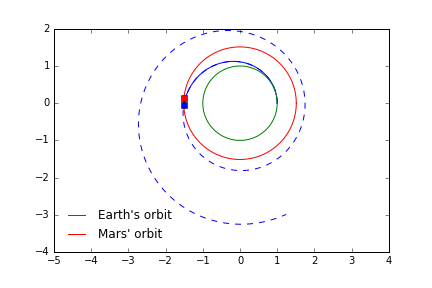
\includegraphics[scale=0.5]{simu.png}
	\caption{\small Simulation of the trajectory of the sail. The Sun is at the origin and axes are in AU. The blue squared represents the sail when reaching Mars' orbit, and the red square, Mars at this same time.}
	\label{fig:simu}

\end{figure} 
The simulation in  \autoref{fig:simu} has been run under the assumption that the initial radial velocity of the sail is nule. This idea, supported by litterature and flight plans of previous missions, can be explained arguing the sole effect of the escape velocity the sail has is that of counteracting Earth's pull.


In a first attempt of reaching Mars from the initial proposed configuration and without a need of manouvers, simulations have been run in order to find a proper sail angle and flight plan. \autoref{fig:espirals} shows some representative results of such simulations. As it has been mentioned before, gravitational pull from Mars has not been taken into account when running the simulations, since it is thought not to be strong enough to have considerable effects on the trajectory. However, in trajectories passing close enough to the planet, as such presented in \autoref{fig:espirals}, the attractive force of gavity will eventually be important enough to take into account, which will, on the one hand, enable the space craft to reach the target, but will also affect on its relative velocity to in. In an attempt of approximating this velocity, we first simulate the relative speed between both bodies at the time plotted.

Assuming the trajectories of Mars and the space craft to be tangential in the first three plots in Figure 5, as they are in good aproximation, one gets relative speeds of \SI{-8,5}{km\cdot s^{-1}}, \SI{-3.5}{km\cdot s^{-1}}  and \SI{-4.7}{km\cdot s^{-1}}, meaning the planet is reachisg the sail. As it has been said, this results do not consider Mars' pull,  but they are believed to be suitable for the start of a landing maneuver in the cases where the distance between both bodies allow it.



\begin{figure}
	\centering
	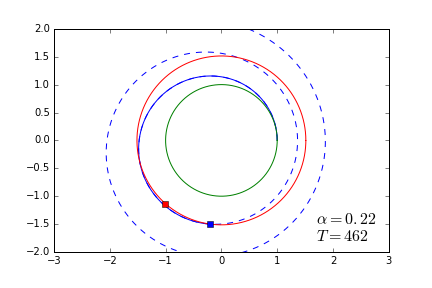
\includegraphics[scale=0.5]{simulacio1.png}
	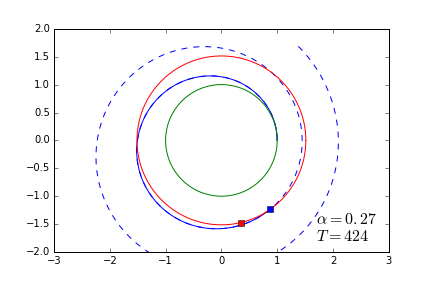
\includegraphics[scale=0.5]{simulacio2.png}
	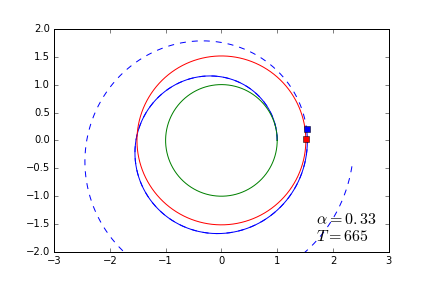
\includegraphics[scale=0.5]{simulacio3.png}
	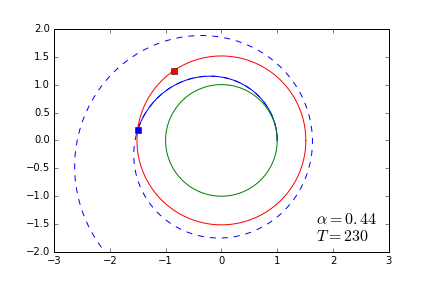
\includegraphics[scale=0.5]{simulacio4.png}
	\caption{Simulation of sail trajectories for different sail angles, $\alpha$, in radians. T indicates the time of flight, in days. The green orbit is Earth's, and the red one is Mars'. The blue square indicates the intersection between Mars' orbit and the trajectory of the space craft, and the red square indicates the position of Mars at this exact time. Axes in AU.}
	\label{fig:espirals}
\end{figure}
\subsection{Sail steering}
In the last section it has been shown that it is quite hard to arrive to Mars orbit at a close position to the planet. This raises some issues regarding not only the possibility of encountering Mars but also whether craft speed is safe enough or not. The idea that is given in the section consists in trying to stabilize the solar sail at Mars orbit. Being succesful with this would implie a similar velocity to Mars orbital one, and moreover, the guarantee of finding the planet since phase difference can be corrected by changing launching positions as explained in Section 3.1.2. 
\begin{figure}
	\centering
	\label{fig:maniobres}
	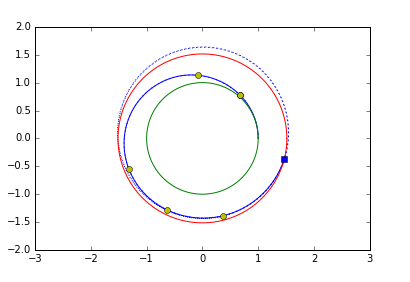
\includegraphics[scale=0.55]{Maniobres.png}
	\caption{Trajectory of the sail with the manoeuvres required to stabilize the orbit, yellow dots. Spacecraft as a blue square in the moment of crossing Mars orbit for the first time. Axes in AU.}
\end{figure}

This will be ensured by making $\alpha$, which determines the force acting on the sail, a function of time. An ideal model would consider this $\alpha(t)$ as a continous function of time and this can be done using similar methods to those used in \cite{xinos}. Nevertheless, due to the complexity of simulations, in this survey it is shown $\alpha$ as a function which is constant in different intervals of time. As a consequence, the model suggests that making an approach to Mars orbit is possible with few manoeuvres, this is, with few changes of $\alpha$. Obviously, one must not forget that the orbit achieved is not the same as Mars one, but it is actually really close. Notice, moreover, that the last manoeuvre sets $\alpha=0$ something which will imply a resulting force characteristic of a central force, a bit different of the gravitational one because of the sun light orthogonal incidence. Calculations give a really close proximity between Mars and the craft within 5 years since the launching moment with initial conditions, and a relative speed of $2$km/s, something that will ensure a safe landing. Simulation also suggests another monoeuvre would be needed after some years of orbit if it was wanted to mantain it. Even though the aim of this approach was not to land on Mars but to orbit like it, since, changing initial positions in real life would assure the desired landing.

Furthermore, it is required to know $\alpha(t)$ in order to design the flight plan represented in \autoref{fig:maniobres}. This is shown in \autoref{fig:escaleta}. Data of this manoeuvres is inspired once again in \cite{xinos}.


\begin{figure}
	\label{fig:escaleta}
	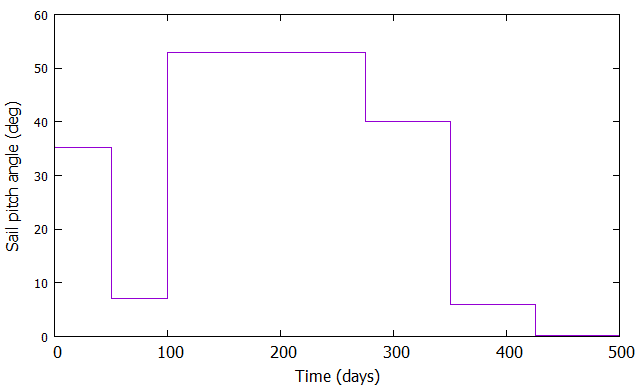
\includegraphics[scale=0.35]{cocu.png}
	\caption{Representation of the manoeuvres needed to stabilize the orbit.}
\end{figure}
\clearpage
\bibliographystyle{ieeetr}
\bibliography{UphysicscNotes}

\onecolumn
\appendix
\section{Python code for numerical solution}
\begin{minted}[breaklines=true,obeytabs=true,tabsize=2]{python}
	#Simulation of the sail trajectory
	
	import numpy as np
	%matplotlib inline
	import matplotlib.pyplot as plt
	from scipy.integrate import odeint
	
	ar=0.000645
	ag=0.0059288888
	alpha=       #Free to change
	a1=ar*np.cos(alpha)**3-ag
	a2=ar*np.sin(alpha)*np.cos(alpha)**2
	r0=1.5*10**11
	theta0=0
	u0=0
	v0=np.sqrt(2*10**30*6.67*10**(-11)/(1.5*10**11))
	
	def simu(y,t):
		r,theta,u,v=y
		dydt=[u,v/r,a1*(r0/r)**2+v**2/r,a2*(r0/r)**2-u*v/r]
		return dydt
	
	y0=[r0,theta0,u0,v0]
	t=np.linspace(0,380*3600*24*5,100000)
	sol=odeint(simu,y0,t)
	
	rsol=[]
	thsol=[]
	usol=[]
	vsol=[]
	for i in range (0,len(sol)):
			rsol.append(sol[i][0])
			thsol.append(sol[i][1])
			usol.append(sol[i][2])
			vsol.append(sol[i][3])
		
	time=[]      #Find time it reaches Mars' orbit
	for i in range (30000,len(sol2)):
			if rsol2[i]<=(2.27+0.1)*10**11 and rsol2[i]>=(2.27-0.1)*10**11:
					time.append((i,rsol2[i]))
	time
	
	a=t2[]  #Introduce manually time taken from above
	
	t2=np.linspace(0,a,100000)  #trajectory until Mars' orbit
	sol2=odeint(simu2,y0,t2)
	rsol2=[]
	thsol2=[]
	usol2=[]
	vsol2=[]
	for i in range (0,len(sol)):
			rsol.append(sol[i][0])
			thsol.append(sol[i][1])
			usol.append(sol[i][2])
			vsol.append(sol[i][3])
	
	
	x=[]					#Hypothetical trajectory
	y=[]
	for i in range (0,len(sol)):
			x.append(rsol[i]*np.cos(thsol[i])/(1.5*10**11))
			y.append(rsol[i]*np.sin(thsol[i])/(1.5*10**11))
	x2=[]				#Trajectort unil Mars' orbit
	y2=[]
	for i in range (0,len(sol2)):
			x2.append(rsol2[i]*np.cos(thsol2[i])/(1.5*10**11))
			y2.append(rsol2[i]*np.sin(thsol2[i])/(1.5*10**11))
	
	xmf=2.27*10**11*np.cos(1.088*10**(-7)*a)/(1.5*10**11)  #Position of Mars when reaching orbit
	ymf=2.27*10**11*np.sin(1.088*10**(-7)*a)/(1.5*10**11)
	
	xnf=rsol[100000-1]*np.cos(thsol[100000-1])/(1.5*10**11)  #Position of sail when reaching orbit
	ynf=rsol[100000-1]*np.sin(thsol[100000-1])/(1.5*10**11)
	
	def frange(start, end=None, inc=None):
			if end == None:
					end = start + 0.0
					start = 0.0
	
			if inc == None:
					inc = 1.0
	
		L = []
		while 1:
				next = start + len(L) * inc
				if inc > 0 and next >= end:
						break
				elif inc < 0 and next <= end:
						break
				L.append(next)
	
		return L
	
	xm=[]   #Mars orbit
	ym=[]
	for i in frange(0,2*np.pi,0.01):
			xm.append(2.27*10**11*np.cos(i)/(1.5*10**11))
			ym.append(2.27*10**11*np.sin(i)/(1.5*10**11))
	
	xt=[]  #Earth's orbit
	yt=[]
	for i in frange(0,2*np.pi,0.01):
			xt.append(1.5*10**11*np.cos(i)/(1.5*10**11))
			yt.append(1.5*10**11*np.sin(i)/(1.5*10**11))
	
	
	plt.plot(x,y)			#plot results
	plt.plot(x,y,'--',color='blue')
	plt.plot(xt,yt)
	plt.plot(xm,ym)
	plt.axis('equal')
	plt.plot([xmf],[ymf],'rs')
	plt.plot([xnf],[ynf],'bs')

	
\end{minted}

\end{document}

